%!TEX root = ../report.tex
\section{Results}
We have implemented the methods as described in the Implementation section.
Our project is not quite done, but the first results are visible in figure~\ref{fig:res}


\begin{figure}[!th]
\hrule
\begin{center}
\vspace*{2ex}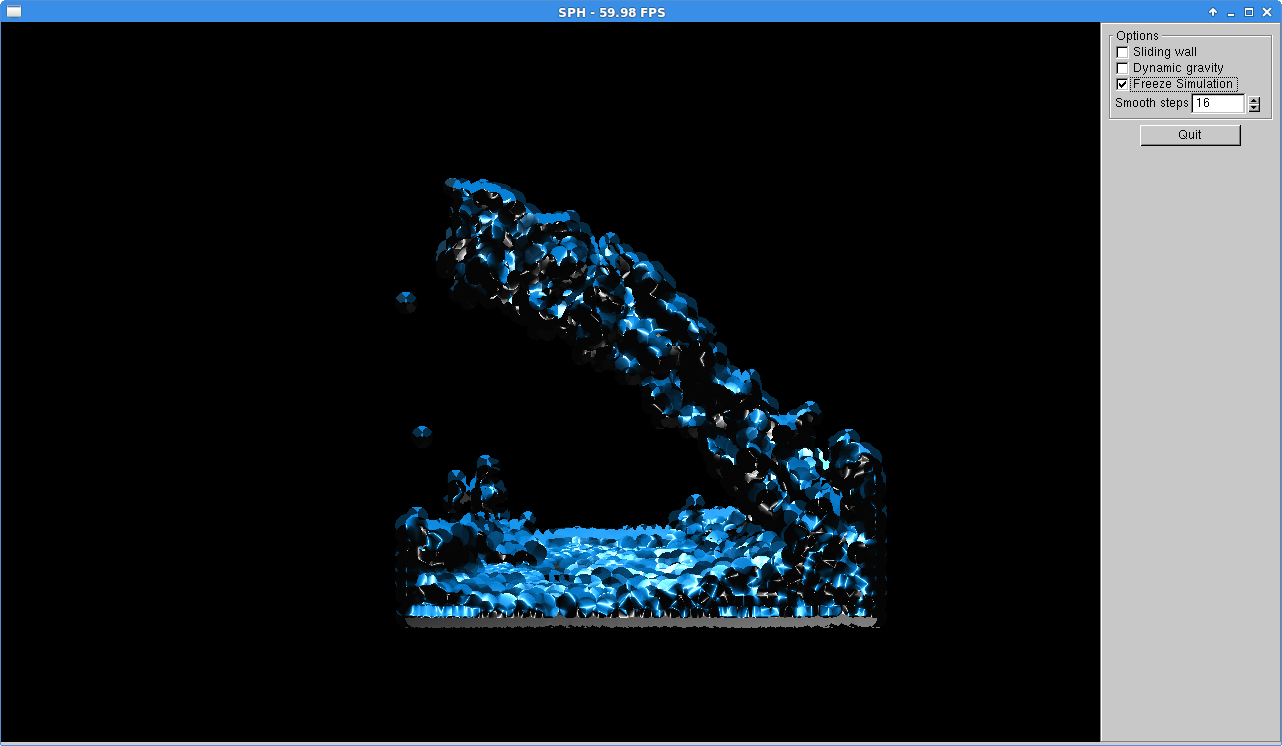
\includegraphics[width=0.48\textwidth]{pictures/colors.png}
\end{center}
\caption{Shaded results}
\label{fig:res} 
\vspace*{2ex}
\hrule
\end{figure}